\documentclass{article}
\usepackage{caption, float, graphicx, subcaption}
\usepackage[dvipsnames]{xcolor}
\usepackage{listings}
\captionsetup[table]{skip=1em}
\usepackage[margin=1in]{geometry}

\lstset{escapeinside={(*@}{@*)}}
\lstdefinestyle{R}
{
	language=R,
	basicstyle=\small\ttfamily,
	numbers=left,
	backgroundcolor=\color{white},
	frame=single,
	rulecolor=\color{black},
	tabsize=1,
	breaklines=true,
	breakatwhitespace=false,
	keywordstyle=\color{Blue},
	commentstyle=\color{Green},
	stringstyle=\color{ForestGreen}
}


\title{ESE 326: Final Project}
\author{Eric Stewart \& Gabriel Minton}
\date{November 2024}


\begin{document}

\maketitle
\tableofcontents

\color{red}
\vskip 1em
!!! All content must end on page 6 !!!
\color{black}

\newpage

\section{Introduction}
The main objective of this project involoved R's built-in dataset, Iris. This dataset contains measurements of 150 iris flowers, from three species: Setosa, Versicolor, and Virginica. Each specimen has measurements of petal length, petal width, sepal length, and sepal width. Through
graphical exploration and mathematical analysis, the reseachers determine whether
there are clear rules as to which of these features can determine the species of a
given specimen. Through these two forms of analysis, the researchers will show if and how the three species of iris flowers can be differentiated by the four features.


\section{Methods}

\subsection{Exploratory Analysis}
% explain how to do analysis and what it will show 
%Section 2: Methods (general description on the methods used to carry out exploratory data
%analysis, confidence interval estimate, and hypothesis test).
%Section 3: Results and Observations (present the results obtained in the form of tables and
%figures)

Exploratory data analysis is meant for betterunderstanding and visualizing the data. This will also allow for researchers to form hypotheses and find patterns. Later in this report, these patterns will be proven or disproven given the evidence found from the mathematical Inference analysis.

For this project, the researchers have created multiple graphs showing how the features of the Iris dataset are separated between species. The first set of graphs, Figure~\ref{fig:iris_colored}, plots pairs of features separated by species. These plots begin to show separation between the features of the different species. This is not enough data to concretely show that there exist statistical differences between the features of each species. Next, the researchers created boxplots for each feature. These, shown in Figure~\ref{fig:feature_boxplots}, more discretely show separation between the three Iris species. These findings will be discussed further in the following sections.


\subsection{Confidence Interval Estimate}

A confidence interval estimate is a range of values, derived from sample data, that is likely to contain a true population parameter with a specified level of confidence. In this case, the sample data consist of the various parameters of the Iris dataset, with the confidence interval estimates specifically focused on their sample means. Since the sample size is large (greater than 30), the sample means will follow a normal distribution according to the Central Limit Theorem. This justifies the use of the Z-distribution for confidence interval estimation as seen in Eq. \ref{eq:ci}.

\begin{equation}
\bar{X} \sim N\left(\mu, \frac{S^2}{n}\right) \quad \Rightarrow \quad \frac{\bar{X} - \mu}{S/\sqrt{n}} \sim N(0,1) \label{eq:ci}
\end{equation}

After establishing that the sample means follow a normal distribution, the confidence intervals for each parameter in the Iris datset were caluculated using R. For each parameter, the corresponding confidence interval provides a range of values that are likely to contain the true population mean with a specified confidence level. These intervals are then used to assess the variability and reliability of the sample estimates. 

\subsection{Hypothesis Test}

The next step was to use a hypothesis test to compare the means of two population samples. Since the variance is unknown for each population, the test for equality of variances was conducted first using a p-value test on an f-distribution. If the variances are found to be equal ($\sigma_1 = \sigma_2$), a pooled variance is used as seen in Eq. \ref{eq:pool_sample_variance}.

\begin{equation}
	{S_p}^2 = \frac{(n_1 - 1) {S_1}^2 + (n_2 -1) {S_2}^2}{n_1 + n_2 -2}
	\label{eq:pool_sample_variance}
\end{equation}

This result also leads to the test statistic following a t-distribution with degrees of freedom equivalent to $n_1+n_2-2$, where $n_1$ and $n_2$ are the sample sizes for each population. The test statistic, calculated using the pooled variance, is given by Eq. \ref{eq:t-test_equal}

\begin{equation}
	\frac{(\bar{X}_1 - \bar{X}_2) - (\mu_1 - \mu_2)}{\sqrt{{S_p}^2
	\left(\frac{1}{n_1} + \frac{1}{n_2} \right)}} \sim T_{n_1 + n_2 -2}
	\label{eq:t-test_equal}
\end{equation}

If the variances are found to be not equal ($\sigma_1 \neq \sigma_2$), a different test statistic must be used. The test statistic, as shown in Eq. \ref{eq:t-test_unequal}, will follow a t-distribution with degrees of freedom $\gamma$. 

\begin{equation}
	\frac{(\bar{X}_1 - \bar{X}_2) - (\mu_1 - \mu_2)}{\sqrt{\frac{S_1^2}{n_1} +
	\frac{S_2^2}{n_2}}} \sim T_\gamma
	\label{eq:t-test_unequal}
\end{equation}

When the variances of the two populations are unequal, the degrees of freedom ($\gamma$) are not simple the sum of the sample sizes minus two. Instead, the degrees of freedom are calculated using Eq. \ref{eq:gamma_unequal}.

\begin{equation}
	\gamma = \frac{\left(\frac{S_1^2}{n_1} + \frac{S_2^2}{n_2}
	\right)^2}{\frac{\left(\frac{S_1^2}{n_1} \right)^2}{n_1 - 1} +
	\frac{\left(\frac{S_2^2}{n_2} \right)^2}{n_2 - 1}}
	\label{eq:gamma_unequal}
\end{equation}

After calculating the appropriate test statistic for the hypthesis test, the next step is to determine to reject or fail to reject the null hypothesis. The p-value test was used for this decision. If the p-value is less than the significance level $\alpha$, the null hypthesis is rejected. If the p-value is greater than or equal to the signaificance level $\alpha$, the null hypothesis is not rejected.

\section{Results and Observations}
\subsection{Exploratory Analysis}

Figure~\ref{fig:feature_boxplots} depicts the 6 pairings of the four features. These features are petal length, petal width, sepal length, and sepal width. Several images are jumbled together, showing that the species have no statistical difference for that feature. For example, take the Sepal Length column. There is not a distinct horizontal separation between the colored species. This means that the sepal length is roughly the same for each species of iris. Similarly, the Sepal Width column shows that there is not a significant statistical separation between species for that feature.
The Petal Length subplots show that Versicolor and Virginica are close, but the Setosa points have much smaller values. This could mean that Setosa is statistically smaller than the other two species. This is supported by Figure~\ref{fig:box_petal_length}. Likewise, the Petal Width subplots show the Versicolor and Virginica points very close, though perhaps still statistically different. The Setosa plots definitely have smaller values than those of the Versicolor and Virginica datapoints. The best plot to see these differences is the Petal Length/ Petal Width plot(s), as the blue setosa group is away from the green and red Versicolor and Virginica groups.

The researchers also prepared a set of boxplots (Figure~\ref{fig:feature_boxplots}). As a property of boxplots, the vertical separation represents a statistical difference between samples. Figures~\ref{fig:box_petal_length}~and~\ref{fig:box_petal_width} show a significant amount of difference between the species for Petal Lengths and Petal Widths, respectively. For each of these features, there is a clear separation of the species. Setosa has the smallest petals, with Versicolor and Virginica being larger. As expected, this is the same result as found from Figure~\ref{fig:iris_colored}. The boxes for Sepal Length show the same pattern, though the Versicolor and Virginica boxes have some overlap (Figure~\ref{fig:box_sepal_length}). Figure~\ref{fig:box_sepal_width} changes the previous pattern of Setosa having the smallest features. This subplot also has overlap for all three boxes, meaning there is no statistical difference between species for sepal width. This is reflected in the Sepal Width column of Figure~\ref{fig:iris_colored}, where all three species populate the same horizontal region.


\begin{figure}[H]
	\centering
	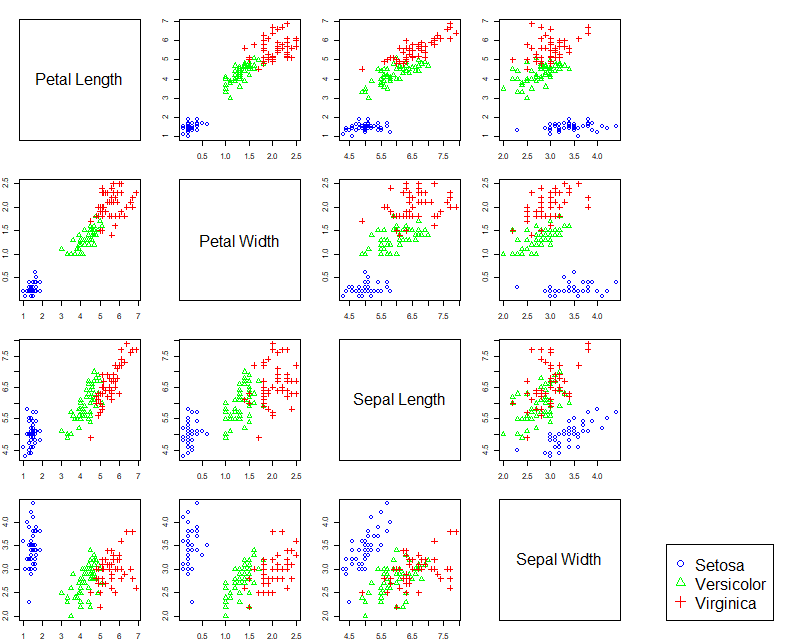
\includegraphics[width=0.7\textwidth]{iris_colored.png}
	\caption{A visualization of the Iris dataset showing scatterplots of each pair
	of the features.}
	\label{fig:iris_colored}
\end{figure}

% Show the feature boxplots together
\begin{figure}[H]
	\centering
	\begin{subfigure}{0.3\textwidth}
		\centering
		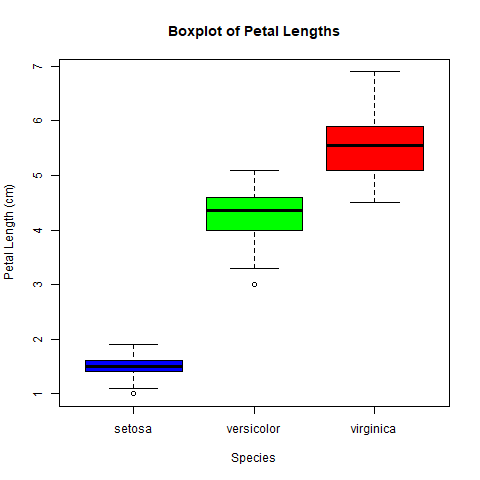
\includegraphics[width=\linewidth]{box_petal_length.png}
		\caption{Petal Lengths}
		\label{fig:box_petal_length}
	\end{subfigure}%
	\begin{subfigure}{0.3\textwidth}
		\centering
		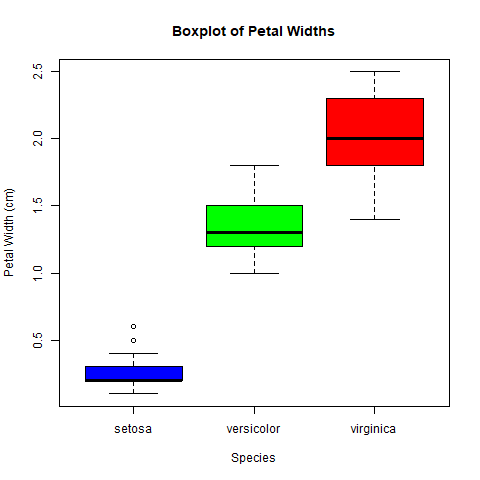
\includegraphics[width=\linewidth]{box_petal_width.png}
		\caption{Petal Widths}
		\label{fig:box_petal_width}
	\end{subfigure}\\
	\begin{subfigure}{0.3\textwidth}
		\centering
		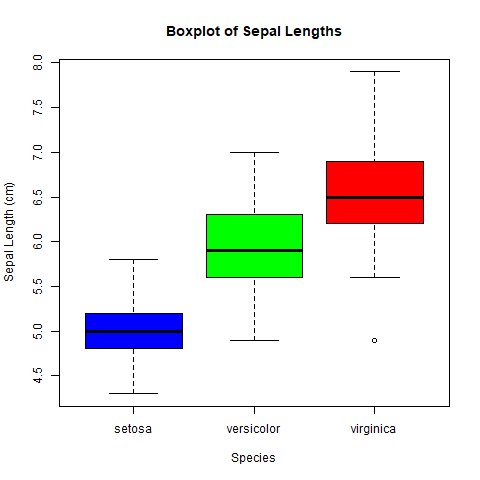
\includegraphics[width=\linewidth]{box_sepal_length.png}
		\caption{Sepal Lengths}
		\label{fig:box_sepal_length}
	\end{subfigure}
	\begin{subfigure}{0.3\textwidth}
		\centering
		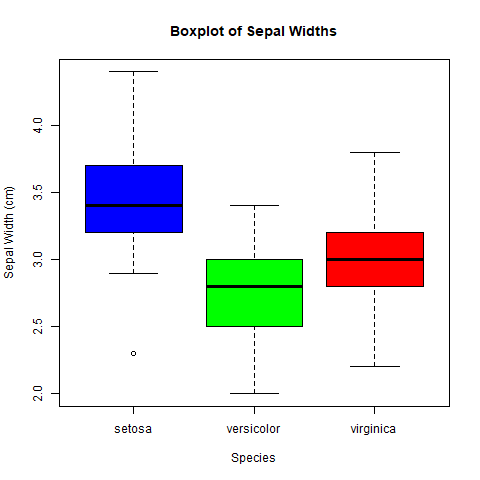
\includegraphics[width=\linewidth]{box_sepal_width.png}
		\caption{Sepal Widths}
		\label{fig:box_sepal_width}
	\end{subfigure}\\
	\caption{Boxplots for each of the four features.}
	\label{fig:feature_boxplots}
\end{figure}



\subsection{Inference Analysis}

The analysis begins with visualizing the distributations of the petal length and petal width using histograms. This allows for an initial assessment of the underlying patters and potential differences betweent the groups before performing statistical tests. Similar to the exploritory analysis, it is noticable in Figure \ref {fig:hist_iris} that the virginica species has a larger petal legnth and width with a approximant mean of 5.5 cm and 2 cm respectively. The results also show that the setosa species has the smallest petal length and withd with sample means at 1.5 and 0.2 respectively. 

% Show the histogram plot
\begin{figure}[H]
	\centering
	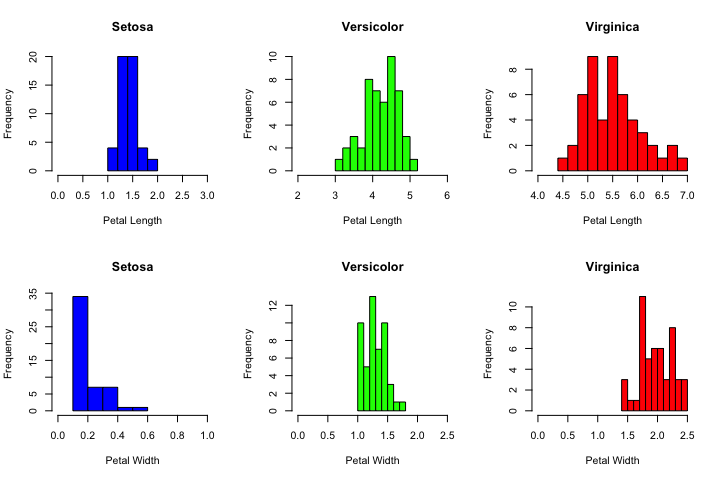
\includegraphics[width=0.7\textwidth]{hist_iris.png}
	\caption{Histograms of Petal lengths and widths for Setosa, Versicolor, and
	Virginica}
	\label{fig:hist_iris}
\end{figure}

The 95\% confidence intervals for the petal lengths of the three iris species were calculated to estimate the population mean for each species. The confidence intervals for petal length were [1.41, 1.51] cm for the Setosa species, [4.13, 4.39] cm for the Versicolor species, and [5.4, 5.7] cm for the Virginica species. These intervals indicate that the petal lengths of each species are distinct from one another, as there is no overlap between the intervals. Although the intervals provide an estimate of the population mean for each species at a 95\% confidence level, they do not conclusively confirm whether the populations are significantly different. A formal hypothesis test would be necessary to make this determination.

Since the population standard devaition ($\sigma$) was unknown for the iris species, a test was conducted to determine whether the variances of the two samples were equal, using a significance level of 0.05. The result of this variance equality test determined the appropriate t-distribution for the subsequent hypothesis test. For the first hypothesis test, the null hypothesis  ($H_0$) stated that the petal length of Virginica iris is larger than or equal to that of Versicolor. The alternative hypothesis ($H_1$) stated that the petal length of Versicolor iris is larger than that of Virginica. The p-value for the variance equality test was 0.259, which greater than the significance level ($\alpha = 0.05$), indicating that it is reasonable to assume the variances of the two populations are equal. Based on this result the t-distribution for the hypothesis test used the pooled vairance, as given in Eq. \ref{eq:t-test_equal}. The resulting p-value for this hypothesis test was 1, indicating that there is no evidence to reject the null hypothesis with a significance value of 0.05. Therefore, it cannot be concluded that the petal length of Versicolor iris is larger than that of Virginica.

 For the second hypothesis test, the null hypothesis ($H_0$) stated that the petal length of Versicolor iris is larger than or equal to that of Setosa iris, while the alternative hypothesis ($H_1$) stated that the petal length of Setosa iris is larger than that of Versicolor. The test for variance equality resulted in a p-value of $6.6\times10^{-11}$, indicating that the variances of the two populations are not equal. As a result, the t-distribution used the test statistic for unequal variances, as described in Eq. \ref{eq:t-test_unequal}. The final p-value for this hypothesis test was 1, showing no evidence to reject the null hypothesis with a significance value of 0.05. Therefore, it cannot be concluded that the petal length of Setosa iris is larger than that of Versicolor. These results align with the exploratory analysis and confidence interval findings, which also indicated differenes in petal lengths among species but did not provide evidence to support the specific claims tested in these hypothesis tests. 

\section{Conclusions}

\color{black}
\newpage
\section{Appendix}

\subsection{Extra Figures and Tables} 
\subsection{R-scripts}
\subsubsection{Exploratory.r}

\begin{lstlisting}[style=R]
# Load packages
library(dplyr)

# Load data
data(iris)
summary(iris)

# Split dataset into different species
names(iris) <- tolower(names(iris))

# Colors:
# Setosa  Versicolor  Virginica
# Blue    Green       Red
# Shapes:
# Circle  Triangle    +
colors <- c('Setosa'='blue', 'Versicolor'='green', 'Virginica'='red')
shapes <- c('Setosa'=1,      'Versicolor'=2,       'Virginica'=3)

# *********************
# PART 1: Plots
# *********************

# IRIS Template
png('iris_gray.png')
plot(iris)
dev.off()

## IRIS Colors
png('iris_colored.png', width = 800, height = 640)
#title()
par(mfrow=c(4, 5), mar=c(2, 2, 2, 2))
plot(x = 0:10, y = 0:10, ann=F, bty='o', type='n', xaxt='n', yaxt='n')
text(x = 5, y = 5, 'Petal Length', cex=2)
plot(iris$petal.width, iris$petal.length, col=colors[iris$species], pch=shapes[iris$species])
plot(iris$sepal.length, iris$petal.length, col=colors[iris$species], pch=shapes[iris$species])
plot(iris$sepal.width, iris$petal.length, col=colors[iris$species], pch=shapes[iris$species])
plot(x = 0:10, y = 0:10, ann=F, bty='n', type='n', xaxt='n', yaxt='n')

plot(iris$petal.length, iris$petal.width, col=colors[iris$species], pch=shapes[iris$species])
plot(x = 0:10, y = 0:10, ann=F, bty='o', type='n', xaxt='n', yaxt='n')
text(x = 5, y = 5, 'Petal Width', cex=2)
plot(iris$sepal.length, iris$petal.width, col=colors[iris$species], pch=shapes[iris$species])
plot(iris$sepal.width, iris$petal.width, col=colors[iris$species], pch=shapes[iris$species])
plot(x = 0:10, y = 0:10, ann=F, bty='n', type='n', xaxt='n', yaxt='n')


plot(iris$petal.length, iris$sepal.length, col=colors[iris$species], pch=shapes[iris$species])
plot(iris$petal.width, iris$sepal.length, col=colors[iris$species], pch=shapes[iris$species])
plot(x = 0:10, y = 0:10, ann=F, bty='o', type='n', xaxt='n', yaxt='n')
text(x = 5, y = 5, 'Sepal Length', cex=2)
plot(iris$sepal.width, iris$sepal.length, col=colors[iris$species], pch=shapes[iris$species])
plot(x = 0:10, y = 0:10, ann=F, bty='n', type='n', xaxt='n', yaxt='n')

plot(iris$petal.length, iris$sepal.width, col=colors[iris$species], pch=shapes[iris$species])
plot(iris$petal.width, iris$sepal.width, col=colors[iris$species], pch=shapes[iris$species])
plot(iris$sepal.length, iris$sepal.width, col=colors[iris$species], pch=shapes[iris$species])
plot(x = 0:10, y = 0:10, ann=F, bty='o', type='n', xaxt='n', yaxt='n')
text(x = 5, y = 5, 'Sepal Width', cex=2)
plot(x = 0:10, y = 0:10, ann=F, bty='n', type='n', xaxt='n', yaxt='n')

legend('bottom', legend=c('Setosa', 'Versicolor', 'Virginica'), col=colors, pch=shapes, cex = 2)
dev.off()


# *********************
# PART 2: Boxplots
# *********************

# Sepal Length
png('box_sepal_length.png')
boxplot(sepal.length ~ species, data=iris, col=colors,
        main='Boxplot of Sepal Lengths', xlab='Species', ylab='Sepal Length (cm)')
dev.off()


# Sepal Width
png('box_sepal_width.png')
boxplot(sepal.width ~ species, data=iris, col=colors,
        main='Boxplot of Sepal Widths',
        xlab='Species', ylab='Sepal Width (cm)')
dev.off()

# Petal Length
png('box_petal_length.png')
boxplot(petal.length ~ species, data=iris, col=colors,
        main='Boxplot of Petal Lengths',
        xlab='Species', ylab='Petal Length (cm)')
dev.off()

# Petal Width
png('box_petal_width.png')
boxplot(petal.width ~ species, data=iris, col=colors,
        main='Boxplot of Petal Widths',
        xlab='Species', ylab='Petal Width (cm)')
dev.off()
\end{lstlisting}


\subsubsection{Inference.r}
\begin{lstlisting}[style=R]
data(iris)

# **********************
# Part 1
# **********************

# create graph layout
par(mfrow = c(2, 3))

# petal length histograms

# setosa histogram
hist(iris$Petal.Length[iris$Species == "setosa"],
     main = "Setosa", xlab = "Petal Length", col = "blue",
     breaks = 5, xlim = c(0,3))

# versicolor
hist(iris$Petal.Length[iris$Species == "versicolor"],
     main = "Versicolor", xlab = "Petal Length", col = "green",
     breaks = 10, xlim = c(2,6))

# virginica
hist(iris$Petal.Length[iris$Species == "virginica"],
     main = "Virginica", xlab = "Petal Length", col = "red",
     breaks = 10, xlim = c(4,7))

# petal width histograms

# setosa
hist(iris$Petal.Width[iris$Species == "setosa"],
     main = "Setosa", xlab = "Petal Width", col = "blue",
     breaks = 10, xlim = c(0,1))

# versicolor
hist(iris$Petal.Width[iris$Species == "versicolor"],
     main = "Versicolor", xlab = "Petal Width", col = "green",
     breaks = 10, xlim = c(0,2.5))

# virginica
hist(iris$Petal.Width[iris$Species == "virginica"],
     main = "Virginica", xlab = "Petal Width", col = "red",
     breaks = 10, xlim = c(0,2.5))

# Reset layout
par(mfrow = c(1, 1))


### Comments on the distributions
# Since the sample statistics have unknown population variances and the sample sizes are larger than 30, they follow a normal distribution. 
# Petal length parameters (aproximations from histogram)
# * Setosa
# ** Sample Mean      = 1.5
# ** Sample Variance  = 0.5
# * Versicolor
# ** Sample Mean      = 4.25
# ** Sample Variance  = 0.45
# * Virginica
# ** Sample Mean      = 5.5
# ** Sample Variance  = 0.5
# Petal width parameters
# * Setosa
# ** Sample Mean      = 0.25
# ** Sample Variance  = 0.1
# * Versicolor
# ** Sample Mean      = 1.3
# ** Sample Variance  = 0.2
# * Virignica
# ** Sample Mean      = 2
# ** Sample Variance  = 0.25


# **********************
# Part 2
# **********************

# function to calculate the confidence interval on the mean of a normal distribution with an unknown variance
confidence_interval_unknown_variance <- function(sample, confidence = 0.95) {
  n <- length(sample)
  sample_mean <- mean(sample)
  sample_sd <- sd(sample)
  a <- 1 - confidence
  z <- qnorm(1 - a/2,0,1)
  margin_of_error <- z * sample_sd / sqrt(n)
  lower_bound <- sample_mean - margin_of_error
  upper_bound <- sample_mean + margin_of_error
  return(c(lower_bound, upper_bound))
}

# **********************
# Part 3
# **********************

# calculate the confidence interval using the function
setosa_ci <- confidence_interval_unknown_variance(iris$Petal.Length[iris$Species == "setosa"])
versicolor_ci <- confidence_interval_unknown_variance(iris$Petal.Length[iris$Species == "versicolor"])
virginica_ci <- confidence_interval_unknown_variance(iris$Petal.Length[iris$Species == "virginica"])

# print results
print("Confidence Interval for Petal Length (Setosa):")
cat('Lower Bound:', setosa_ci[1], "\n")
cat('Upper Bound:', setosa_ci[2], "\n")

print("Confidence Interval for Petal Length (Versicolor):")
cat('Lower Bound:', versicolor_ci[1], "\n")
cat('Upper Bound:', versicolor_ci[2], "\n")

print("Confidence Interval for Petal Length (Verginica):")
cat('Lower Bound:', virginica_ci[1], "\n")
cat('Upper Bound:', virginica_ci[2], "\n")

# **********************
# Part 4
# **********************

# confidence intervals
# Setosa has confidence intervals of [1.41, 1.51], which means that with 95 percent confidence the populaiton mean lies within these bounds.
# Versicolorhas confidence intervals of [4.14, 4.39], which means that with 95 percent confidence the populaiton mean lies within these bounds.
# Verginica has confidence intervals of [5.4, 5.7], which means that with 95 percent confidence the populaiton mean lies within these bounds.

# **********************
# Part 5
# **********************

sample1 = iris$Petal.Length[iris$Species == "virginica"]
sample2 = iris$Petal.Length[iris$Species == "versicolor"]
conf_level <- 0.95


mean_hypothesis_test <- function(sample1, sample2, conf_level = 0.95) {
  n1 <- length(sample1)       # size of sample1
  n2 <- length(sample2)       # size of sample2
  mean1 <- mean(sample1)      # sample mean for sample1
  mean2 <- mean(sample2)      # sample mean for sample2
  sd1 <- sd(sample1)          # sample sd for sample1
  sd2 <- sd(sample2)          # sample sd for sample2
  
  ### check for equality in variances by testing H0: sigma1=sigma2 : H1: sigma1 ~= sigma2
  # test statistic
  t_stat <- (sd1^2)/(sd2^2)
  # significance level
  alpha <- 1 - conf_level
  # p value
  p_value <- 2*(1-pf(t_stat,n1,n2))
  
  # sigma values are unknown and equal
  if (p_value > alpha) {
    print("sigma1=simga2")
    # degrees of freedom
    df <- n1 + n2 - 2
    # pooled valiance
    Sp <- ((n1-1)*sd1^2 + (n2-1)*sd2^2)/(n1 + n2 - 2)
    # observed value
    T_obs <- (mean1 - mean2)/(sqrt(Sp*((1/n1) + (1/n2))))
    # p value
    pt_value <- pt(T_obs, df)
    
    # sigma values are unknown and unequal
  } else if (p_value < alpha) {
    print("simga1~=simga2")
    # degree of freedom
    gamma <- (((sd1^2/n1) + (sd2^2/n2))^2) / (((sd1^2/n1)^2 / (n1 - 1)) + ((sd2^2/n2)^2 / (n2 - 1)))
    # observed value
    T_obs <- (mean1 - mean2)/(sqrt(((sd1^2/n1) + (sd2^2/n2))))
    # p value
    pt_value <- pt(T_obs, gamma)
    
  }
  print('variance p value')
  print(p_value)
  print('p value final')
  print(pt_value)
  if (pt_value > alpha) {
    result <- "Accept H0"
  } else if (pt_value < alpha) {
    result <- "Reject H0"
  }
  return(result)
}

# **********************
# Part 6
# **********************

first_test <- mean_hypothesis_test(iris$Petal.Length[iris$Species == "virginica"],
                              iris$Petal.Length[iris$Species == "versicolor"],
                              0.95)
second_test <- mean_hypothesis_test(iris$Petal.Length[iris$Species == "versicolor"],
                                   iris$Petal.Length[iris$Species == "setosa"],
                                   0.95)
print("Petal length of Virginica iris is larger than that of Versicolor")
print(first_test)
print("Petal length of Versicolor iris is larger than that of Setosa")
print(second_test)

# **********************
# Part 7
# **********************

# Petal length of Virginica iris is larger than that of Versicolor
# H0: mu1 >= m2 : H1: mu2 > mu1
# population variance test results in pooled variance (p-vale = 0.259)
# failed to reject null hypothesis because p-value = 1

# Petal length of Versicolor iris is larger than that of Setosa
# H0: mu1 >= m2 : H1: mu2 > mu1
# population variance test results in unequal population vairance (p-value = 6.6e-11)
# failed to reject null hypothesis because p-value = 1

\end{lstlisting}


\end{document}
